\section{Belief Propagation: Interpretation}

\subsection{Introduction}

\begin{definition}{\textbf{(Loopy Propagation)}}
    The joint distribution for \emph{any} graph is given by:
    \begin{equation*}
        P(\mathcal{X}) = \frac{1}{Z}\prod_{\text{nodes } i} f_i(\boldsymbol x_i) \prod_{\text{edges } (ij)} f_{ij}(\boldsymbol x_i, \boldsymbol x_j)
    \end{equation*}
    Message computed recusively with few guarantee of convergence as we have the following message:
    \begin{equation*}
        M_{j\rightarrow i} = \sum_{\boldsymbol x_j} f_{ij}(\boldsymbol x_i, \boldsymbol x_j)f_j(\boldsymbol x_j)\prod_{l \in \operatorname{ne}(j)\backslash\brackc{i}} M_{l\rightarrow j}(\boldsymbol x_j)
    \end{equation*}
    The marginal distribution are approximation in general:
    \begin{equation*}
    \begin{aligned}
        &P(\boldsymbol x_i) \approx b_i(\boldsymbol x_i) \propto f_i(\boldsymbol x_i)\prod_{k\in\operatorname{ne}(i)}M_{k\rightarrow i}(\boldsymbol x_i) \\
        &P(\boldsymbol x_i, \boldsymbol x_j) \approx b_{ij}(\boldsymbol x_i, \boldsymbol x_j) \propto f_{ij}(\boldsymbol x_i, \boldsymbol x_j)f_i(\boldsymbol x_i)f_j(\boldsymbol x_j)\prod_{k\in\operatorname{ne}(i)\backslash \brackc{j}} M_{k\rightarrow i}(\boldsymbol x_i)\prod_{l\in\operatorname{ne}(j)\backslash \brackc{i}}M_{l\rightarrow j}(\boldsymbol x_j)
    \end{aligned}
    \end{equation*}
\end{definition}

\begin{remark}{\textbf{(Dealing with Loops)}}
    There are various way to deal with loop as we have:
    \begin{itemize}
        \item The belief propagation posterior marginal are approximate on all non-tree because over-counted, but converged approximate are frequently found to be good. 
        \item Converge can be seen in: Tree, Graph with single step, Distribution with weak iteraction, Graph with long (and weak) loops, and Gaussian network (variance may also converged).
        \item Damping, as it is a common approach to encorate of EP:
        \begin{equation*}
            M^\text{new}_{i\rightarrow j}(\boldsymbol x_j) = (1-\alpha)M^\text{old}_{i\rightarrow j} + \alpha\sum_{\boldsymbol x_i}f_{ij}(\boldsymbol x_i, \boldsymbol x_j)f_i(\boldsymbol x_i) \prod_{k\in\operatorname{ne}(i)\backslash\brackc{j}}M_{k\rightarrow i}(\boldsymbol x_i)
        \end{equation*}
        \item Variable can be groupped into cliques to improve accuracy: region graph approximate, cluster variable method, and junction graph.
    \end{itemize} 
\end{remark}

\subsection{Message Based EP}

\begin{proposition}{\textbf{(Loopy BP as Message-Based EP)}}
    One can consider the connection between message-based EP and loopy BP, as they are equivalent.
\end{proposition}
\begin{proof}
    Consider the appoximate pairwise factor $\tilde{f}_{ij}$ as product of messages:
    \begin{equation*}
        f_{ij}(\boldsymbol x_i, \boldsymbol x_j) \approx \tilde{f}_{ij}(\boldsymbol x_i, \boldsymbol x_j) = M_{i\rightarrow j}(\boldsymbol x_j)M_{j\rightarrow i}(\boldsymbol x_i)
    \end{equation*}
    Consider the approximation of the factorized distribution:
    \begin{equation*}
    \begin{aligned}
        P(\mathcal{X}) &\approx \frac{1}{Z}\prod_{\text{nodes}(i)}f_i(\boldsymbol x_i) \prod_{\text{edges}(ij)}\tilde{f}_{ij}(\boldsymbol x_i, \boldsymbol x_j) \\
        &= \frac{1}{Z}\prod_{\text{nodes}(i)}\bracka{f_i(\boldsymbol x_i)\prod_{j\in\mathcal{N}(i)}M_{j\rightarrow i}(\boldsymbol x_i)} = \prod_{\text{nodes}(i)}b_i(\boldsymbol x_i)
    \end{aligned}
    \end{equation*}
    with multiple factors for $\boldsymbol x_i$, which we consider the update on EP to be:
    \begin{itemize}
        \item \emph{Deletion}: Consider the following $P(\mathcal{X})$ as we have:
        \begin{equation*}
        \begin{aligned}
            P_{\neg ij}&(X_i, X_j) = \sum_{c \ne i, j} \frac{P(\mathcal{X})}{\tilde{f}(X_i, X_j)} = \sum_{c \ne i, j} \frac{P(\mathcal{X})}{ M_{i\rightarrow j}(\boldsymbol x_j) M_{j\rightarrow i}(\boldsymbol x_i)} \\ 
            &= \frac{1}{\tilde{f}(X_i, X_j)}\sum_{c \ne i, j}f_i(\boldsymbol x_i)f_j(\boldsymbol x_j)\prod_{k\in\mathcal{N}(i)}M_{k\rightarrow i}(\boldsymbol x_i)\prod_{l\in\mathcal{N}(j)}M_{l\rightarrow j}(\boldsymbol x_j) \bracka{\prod_{s\ne i, j} f_s(\boldsymbol x_s) \prod_{t\in\mathcal{N}(s)}  M_{t\rightarrow s} (\boldsymbol x_s) } \\
            &= f_i(\boldsymbol x_i)f_j(\boldsymbol x_j)\prod_{k\in\mathcal{N}(i) \backslash j}M_{k\rightarrow i}(\boldsymbol x_i)\prod_{l\in\mathcal{N}(j)\backslash i}M_{l\rightarrow j}(\boldsymbol x_j)\sum_{c \ne i, j}\bracka{\prod_{s\ne i, j} f_s(\boldsymbol x_s) \prod_{t\in\mathcal{N}(s)}  M_{t\rightarrow s} (\boldsymbol x_s) } \\
            &= f_i(\boldsymbol x_i)f_j(\boldsymbol x_j)\prod_{k\in\mathcal{N}(i) \backslash j}M_{k\rightarrow i}(\boldsymbol x_i)\prod_{l\in\mathcal{N}(j)\backslash i}M_{l\rightarrow j}(\boldsymbol x_j) \\
        \end{aligned}
        \end{equation*}
        \item \emph{Projection}: We consider minimizing the KL-divergence as we have:
        \begin{equation*}
            \brackc{M^\text{new}_{i\rightarrow j}, M^\text{new}_{j\rightarrow i}} = \argmin{M_{i\rightarrow j}, M_{j\rightarrow i}} \operatorname{KL}\brackb{ f_{ij}(\boldsymbol x_i, \boldsymbol x_j) q_{\neg ij}(\boldsymbol x_i, \boldsymbol x_j) \Big\| M_{j\rightarrow i}(\boldsymbol x_i) M_{i\rightarrow j}(\boldsymbol x_j)q_{\neg ij}(\boldsymbol x_i, \boldsymbol x_j) }
        \end{equation*}
        To solve this KL-divergence, this is obvious, as $q_{\neg ij}(\cdot)$ can be factorized and so the minimizer is the marginal between $f_{ij}(\cdot)q_{\neg ij}(\cdot)$, which means that:
        \begin{equation*}
        \begin{aligned}
            M_{i\rightarrow j}^\text{new}(\boldsymbol x_j)q_{\neg ij}(\boldsymbol x_i, \boldsymbol x_j)& = \sum_{\boldsymbol x_j}\bracka{f_{ij}(\boldsymbol x_i, \boldsymbol x_j) f_j(\boldsymbol x_j)\prod_{l\in\mathcal{N}(j)\backslash i}M_{l\rightarrow j}(\boldsymbol x_j) } \underbrace{f_i(\boldsymbol x_i)\prod_{k\in\mathcal{N}(i) \backslash j}M_{k\rightarrow i}(\boldsymbol x_i)}_{q_{\neg ij}(\boldsymbol x_i)} \\
            \implies& M_{i\rightarrow j}^\text{new}(\boldsymbol x_j) = \sum_{\boldsymbol x_j}\bracka{f_{ij}(\boldsymbol x_i, \boldsymbol x_j) f_j(\boldsymbol x_j)\prod_{l\in\mathcal{N}(j)\backslash i}M_{l\rightarrow j}(\boldsymbol x_j) }
        \end{aligned}
        \end{equation*}
        This is the Loopy BP update, and so both of the are equivalent. 
    \end{itemize}
\end{proof}

\begin{remark}{\textbf{(Comments on the Loopy BP and EP)}}
    There are some observation that we can make in the equivalent between loopy BP and EP algorithm:
    \begin{itemize}
        \item Unlike EP, this message based EP doesn't need $2$ separate approximate as we have in the normal EP.
        \item This message based EP is loopy graph can be seen as a more constraint on approximate site and not just exponential family factor but the product of exponential family message. 
        \item On a tree, message forward EP finds the same marginal as standard EP as the messages are calculated the same way. Similarly, the pairwise marginal can be found after converge by compute $\tilde{P}(z_{i - 1}, z_i)$
        \item Factorization still remain valid even when original site lies in the appoximation exponential family already, so the loopy BP can be seen as form of EP. 
        \item This doesn't help us with understanding the convergence property of EP.
    \end{itemize}
\end{remark}

\subsection{Reparameterized on Tree}

\begin{remark}{\textbf{(Tree-Based Representation)}}
    We consider the joint factorization, which can be represented:
    \begin{equation*}
    \begin{aligned}
        P(\mathcal{X}) &= \frac{1}{Z}\prod_{\operatorname{nodes}(i)} f_i(\boldsymbol x_i)\prod_{\operatorname{edges}(ij)} f_{ij}(\boldsymbol x_i, \boldsymbol x_j) \qquad \text{(Undirected Tree)} \\
        &= P(\boldsymbol x_i)\prod_{i\ne r}P(\boldsymbol x_i | \boldsymbol x_{\text{pa}(i)}) \qquad \text{(Directed Rooted Tree)} \\
        &= \prod_{\operatorname{nodes}(i)}P(\boldsymbol x_i)\prod_{\operatorname{edges}(ij)}\frac{P(\boldsymbol x_i, \boldsymbol x_j)}{P(\boldsymbol x_i)P(\boldsymbol x_j)}  \qquad \text{(Pairwise Marginal)} \\
    \end{aligned}
    \end{equation*}
    The last on requires that $\sum_{\boldsymbol x_j}P(\boldsymbol x_i, \boldsymbol x_j) = P(\boldsymbol x_i)$. 
    \begin{itemize}
        \item The unidrected tree isn't unique as if we multiply the factor $f_{ij}(\boldsymbol x_i, \boldsymbol x_j)$ by $g(\boldsymbol x_i)$ and dividing $f_i(\boldsymbol x_i)$ by the same $g(\boldsymbol x_i)$ doesn't change the distribution. 
        \item BP can be seen as iteractive replacement of $f_i(\boldsymbol x_i)$ by local marginal of $p_{ij}(\boldsymbol x_i, \boldsymbol x_j)$ along with corresponding representation of $f_{ij}(\boldsymbol x_i, \boldsymbol x_j)$ (recall the Hugin propagation)
        \item Converged BP on a tree finds $P(\boldsymbol x_i)$ and $P(\boldsymbol x_i, \boldsymbol x_j)$ allowing up to transform the undirected tree to pairwise marginal. 
    \end{itemize}
\end{remark}

\begin{remark}{\textbf{(Reparameterization in Tree)}}
    To consider the tree based reparameterization, we want to transform the representation from undirected tree to pairwise marginal as:
    \begin{equation*}
        \prod_{\operatorname{nodes}(i)} f_i(\boldsymbol x_i)\prod_{\operatorname{edges}(ij)} f_{ij}(\boldsymbol x_i, \boldsymbol x_j) \implies \prod_{\operatorname{nodes}(i)}P(\boldsymbol x_i)\prod_{\operatorname{edges}(ij)}\frac{P(\boldsymbol x_i, \boldsymbol x_j)}{P(\boldsymbol x_i)P(\boldsymbol x_j)}
    \end{equation*}
    We will define the $f^0_{ij} = f_{ij}$, while the singleton factor to be $f^0_1 = p^0_1 = 1$, we consider the following update: The update is based on the fact that we will act on the factors \emph{as if} it is actually representing the probabilities: We will consider such a procedure on a node that has $2$ incoming messages. 
    \begin{itemize}
        \item Starting with joint, where if we multiply it by adjacent factors we get $P(\boldsymbol x_i, \boldsymbol x_j)$ i.e
        \begin{equation*}
            p^{(n)}(\boldsymbol x_i, \boldsymbol x_j) = \frac{1}{Z_{ij}^{(n)}} f^{(n-1)}_i(\boldsymbol x_i)f^{(n-1)}_{ij}(\boldsymbol x_i, \boldsymbol x_j) f^{(n-1)}_j(\boldsymbol x_j)
        \end{equation*}
        \item Finding the marginal, as we have:
        \begin{equation*}
            f^{(n)}_i(\boldsymbol x_i) = p^{(n)}(\boldsymbol x_i) = \sum_{\boldsymbol x_j}p^{(n)}(\boldsymbol x_i, \boldsymbol x_j) = f^{(n-1)}_i(\boldsymbol x_i)\underbrace{\sum_{\boldsymbol x_j} f^{(n-1)}_{ij}(\boldsymbol x_i, \boldsymbol x_j) f^{(n-1)}_j(\boldsymbol x_j)}_{M_{j\rightarrow i}}
        \end{equation*}
        \item To keep the normalization correctly, we divide the message so that the update on one passing giving us normalized term:
        \begin{equation*}
            f^{(n)}_{ij} = \frac{f^{(n-1)}_{ij}(\boldsymbol x_i, \boldsymbol x_j)}{M_{j\rightarrow i}(\boldsymbol x_j)}
        \end{equation*}
        \item We now consider the next step with the next incoming message from node $k$ to node $i$:
        \begin{equation*}
        \begin{aligned}
            p^{(n)}(\boldsymbol x_i, \boldsymbol x_k) &= \frac{1}{Z_{ik}^{(n)}} f^{(n)}_i(\boldsymbol x_i)f^{(n-1)}_{ik}(\boldsymbol x_i, \boldsymbol x_j) f^{(n-1)}_k(\boldsymbol x_j) \\
            &= \frac{1}{Z_{ik}^{(n)}} f^{(n-1)}_i(\boldsymbol x_i)M_{j\rightarrow i}(\boldsymbol x_i) f^{(n-1)}_{ik}(\boldsymbol x_i, \boldsymbol x_k) f^{(n-1)}_k(\boldsymbol x_k) \\
        \end{aligned}
        \end{equation*}
        \item Finding the singleton factor by marginalization
        \begin{equation*}
            f^{(n)}_i(\boldsymbol x_i) = f^{(n-1)}_i(\boldsymbol x_i)M_{j\rightarrow i}(\boldsymbol x_i) \underbrace{\sum_{\boldsymbol x_k}f^{(n-1)}_{ik}(\boldsymbol x_i, \boldsymbol x_k) f^{(n-1)}_k(\boldsymbol x_k)}_{M_{k\rightarrow i}}
        \end{equation*}
        \item And so, the normalization correction on the joint factor is:
        \begin{equation*}
            f^{(n)}_{ik} = \frac{f^{(n-1)}_{ik}(\boldsymbol x_i, \boldsymbol x_k)}{ M_{k\rightarrow i}(\boldsymbol x_i) }
        \end{equation*}
    \end{itemize}
    We perform this update throughout the tree, which we do it in forward (e.g $i\rightarrow j$) and backward (e.g $j\rightarrow i$) manner, which gives us:
    \begin{equation*}
    \begin{aligned}
        &f^{(\infty)}_i(\boldsymbol x_i) = \prod_{j\operatorname{ne}(i)}M_{j\rightarrow i}(\boldsymbol x_i) = P(\boldsymbol x_i) \\
        &\begin{aligned}[t]
            f^{(\infty)}_{ij}(\boldsymbol x_i, \boldsymbol x_j) &= \frac{f_{ij}(\boldsymbol x_i, \boldsymbol x_j)}{M_{j\rightarrow i}(\boldsymbol x_i)M_{i\rightarrow j}(\boldsymbol x_j)} \\
            &= \frac{\prod_{k \in \operatorname{ne}(i)\backslash j}M_{k\rightarrow i}f_{ij}(\boldsymbol x_i, \boldsymbol x_j)\prod_{l \in \operatorname{ne}(j)\backslash i}M_{l\rightarrow i}(\boldsymbol x_j)}{\prod_{k \in \operatorname{ne}(i)\backslash j}M_{k\rightarrow i} M_{j\rightarrow i}(\boldsymbol x_i)M_{i\rightarrow j}(\boldsymbol x_j) \prod_{l \in \operatorname{ne}(j)\backslash i}M_{l\rightarrow i}(\boldsymbol x_j) } \\
            &= \frac{\prod_{k \in \operatorname{ne}(i)\backslash j}M_{k\rightarrow i}f_{ij}(\boldsymbol x_i, \boldsymbol x_j)\prod_{l \in \operatorname{ne}(j)\backslash i}M_{l\rightarrow i}(\boldsymbol x_j)}{\prod_{k \in \operatorname{ne}(i)}M_{k\rightarrow i} \prod_{l \in \operatorname{ne}(j)}M_{l\rightarrow i}(\boldsymbol x_j) } \\
            &= \frac{P(\boldsymbol x_i, \boldsymbol x_j)}{P(\boldsymbol x_i)P(\boldsymbol x_j)}
        \end{aligned}
    \end{aligned}
    \end{equation*}
    the equation follows from the result from belief propagation.This kind of reparameterization allows us to avoid double counting, which is essentially a book-keeping method, espescially the normalizing part (there will be a case where the factor cancel with unnecessary message from singleton factor, as intended). 
\end{remark}

\begin{remark}{\textbf{(Comments on the BP on non-tree)}}
    If this converges in a non-tree setting, then we have locally consistent belief i.e:
    \begin{equation*}
        p(\mathcal{X}) \propto \prod_i b(\boldsymbol x_i) \prod_{ij}\frac{b(\boldsymbol x_i, \boldsymbol x_j)}{b(\boldsymbol x_i)b(\boldsymbol x_j)} \quad \text{ such that } \quad \sum_{\boldsymbol x_j}b(\boldsymbol x_i, \boldsymbol x_j) = b(\boldsymbol x_i)
    \end{equation*}
    But it doesn't need to be globally consistent:
    \begin{equation*}
        \sum_{\mathcal{X}_{\neg i}}\bracka{\prod_i b(\boldsymbol x_i) \prod_{ij}\frac{b(\boldsymbol x_i, \boldsymbol x_j)}{b(\boldsymbol x_i)b(\boldsymbol x_j)}} \ne b(\boldsymbol x_i)
    \end{equation*}
    This kind of marginal is called \emph{pseudo-marginal}. 
\end{remark}

\begin{remark}{\textbf{(Message Schedule Scheme)}}
    We consider update the belief on each \emph{subtree} of the graph and passing message on each subtree, looping through all the subtree until converge:
    \begin{figure}[H]
        \centering
        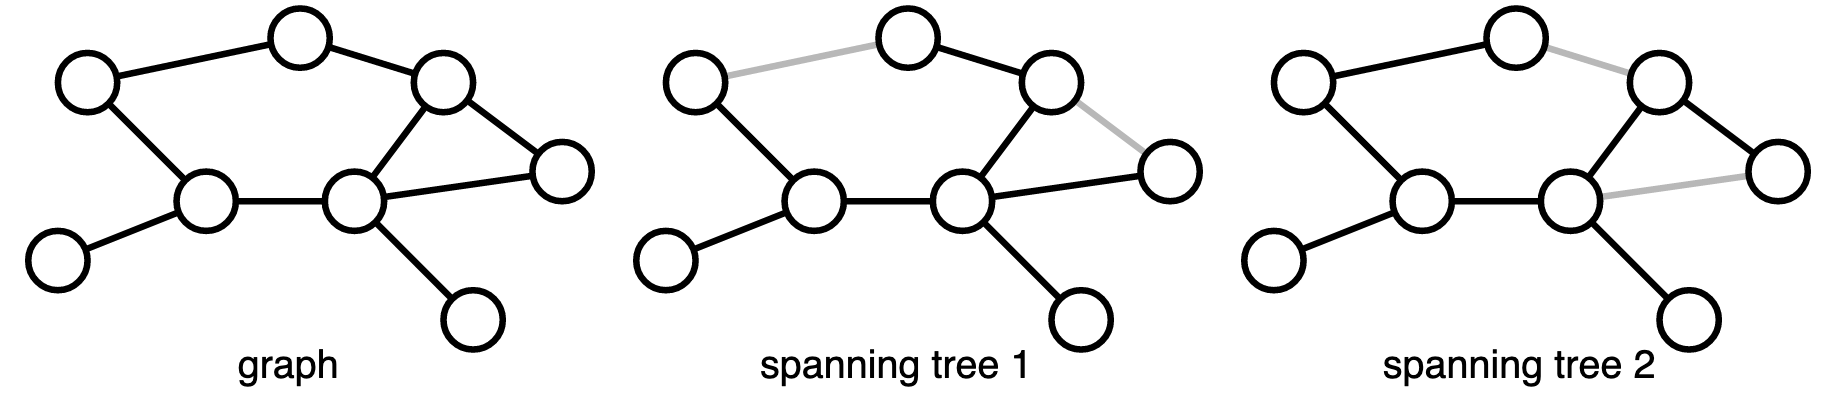
\includegraphics[width=10cm]{img/img16.png}
    \end{figure}  
    And, we now that the following updates steps:
    \begin{equation*}
    \begin{aligned}
        P(\mathcal{X}) 
        &= \frac{1}{Z}\prod_{\operatorname{nodes}(i)} f^{(0)}_i(\boldsymbol x_i)\prod_{\operatorname{edges}(ij)} f^{(0)}_{ij}(\boldsymbol x_i, \boldsymbol x_j) \\
        &= \frac{1}{Z}\prod_{\operatorname{nodes}(i) \in T_1} f^{(0)}_i(\boldsymbol x_i)\prod_{\operatorname{edges}(ij) \in T_1} f^{(0)}_{ij}(\boldsymbol x_i, \boldsymbol x_j)\bracka{\prod_{\operatorname{edges}(ij) \not\in T_1} f^{(0)}_{ij}(\boldsymbol x_i, \boldsymbol x_j)} \\
        &\text{(Update)} \\
        &= \frac{1}{Z}\prod_{\operatorname{nodes}(i) \in T_1} f^{(1)}_i(\boldsymbol x_i)\prod_{\operatorname{edges}(ij) \in T_1} f^{(1)}_{ij}(\boldsymbol x_i, \boldsymbol x_j)\bracka{\prod_{\operatorname{edges}(ij) \not\in T_1} f^{(1)}_{ij}(\boldsymbol x_i, \boldsymbol x_j)} \\
        &\text{(Next Tree)} \\
        &= \frac{1}{Z}\prod_{\operatorname{nodes}(i) \in T_2} f^{(1)}_i(\boldsymbol x_i)\prod_{\operatorname{edges}(ij) \in T_2} f^{(1)}_{ij}(\boldsymbol x_i, \boldsymbol x_j)\bracka{\prod_{\operatorname{edges}(ij) \not\in T_2} f^{(1)}_{ij}(\boldsymbol x_i, \boldsymbol x_j)} \\
        &\cdots
    \end{aligned}
    \end{equation*}
    where we have, when we got a new tree, 
    \begin{equation*}
        f^{(1)}_i(\boldsymbol x_i) = P^{T_1}(\boldsymbol x_i)\qquad f^{(1)}_{ij}(\boldsymbol x_i, \boldsymbol x_j) = \frac{P^{T_1}(\boldsymbol x_i, \boldsymbol x_j)}{P^{T_1}(\boldsymbol x_i)P^{T_2}(\boldsymbol x_j)} 
    \end{equation*}
    If the process converges, suppose it converge to:
    \begin{equation*}
        P(\mathcal{X}) = \frac{1}{Z}\prod_{\operatorname{nodes}(i)} f_i^{(\infty)}(\boldsymbol x_i)\prod_{\operatorname{edges}(ij)} f_{ij}^{(\infty)}(\boldsymbol x_i, \boldsymbol x_j)
    \end{equation*}
    where for any tree $T$ in the graph, we have:
    \begin{equation*}
        f_i^{(\infty)} = P^T(\boldsymbol x_i)\qquad f_{ij}^{(\infty)} = \frac{P^T(\boldsymbol x_i, \boldsymbol x_j)}{P^T(\boldsymbol x_i)P^T(\boldsymbol x_j)}
    \end{equation*}
    This means that the local marginal of all subtree are consistent with each other, and the pseudo-marginal is valid belief of any of the subtree, as this is stronger constriant. 
\end{remark}

\subsection{Bathe Free Energy}

\begin{remark}{\textbf{(Introduction to Bathe Free Energy)}}
    In reparameterization view, BP solves for marginal belief $b_{ij}(\boldsymbol x_i, \boldsymbol x_j)$ and $b_i(\boldsymbol x_i) = \sum_{\boldsymbol x_j}b_{ij}(\boldsymbol x_i, \boldsymbol x_j)$  such that:
    \begin{equation*}
        P(\mathcal{X}) \propto \prod_if_i(\boldsymbol x_i)\prod_{ij}f_{ij}(\boldsymbol x_i, \boldsymbol x_j) \propto \prod_ib_i(\boldsymbol x_i)\prod_{ij}\frac{b_{ij}(\boldsymbol x_i, \boldsymbol x_j)}{b_i(\boldsymbol x_i)b_j(\boldsymbol x_j)}
    \end{equation*}
    Loopy BP is a set of fixed point equation for finding stationary of an objective function called Bathe free energy, which is defined in terms of locally consistent belief (pseudo-marginal) $b_i\ge0$ and $b_{ij}\ge0$ such that:
    \begin{equation*}
        \sum_{\boldsymbol x_i} b_i(\boldsymbol x_i) = 1 \qquad \sum_{\boldsymbol x_j}b_{ij}(\boldsymbol x_i, \boldsymbol x_j) = b_i(\boldsymbol x_i)
    \end{equation*}
\end{remark}

\begin{definition}{\textbf{(Bathe Free Energy)}}
    We define it in the form of:
    \begin{equation*}
        \mathcal{F}_\text{bathe}(b) = \mathcal{E}_\text{bathe}(b) + \mathcal{H}_\text{bathe}(b) 
    \end{equation*}
    Both terms are approximated so that it corresponds to variational likelihood terms:
    \begin{itemize}
        \item Bathe average energy is the expected log-joint evaluate as though the pseudomarginal were correct:
        \begin{equation*}
            \mathcal{E}_\text{bathe}(b) = \sum_i\sum_{\boldsymbol x_i} b_i(\boldsymbol x_i)\log f_i(\boldsymbol x_i) + \sum_{ij}\sum_{\boldsymbol x_i\boldsymbol x_j} b_{ij}(\boldsymbol x_i, \boldsymbol x_j)\log f_{ij}(\boldsymbol x_i, \boldsymbol x_j)
        \end{equation*}
        \item Bathe entropy is the sum of pseudomarginal entropies corrected for pairwise (pseudo-)interaction, but neglecting higher-order dependence:
        \begin{equation*}
        \begin{aligned}
            \mathcal{H}_\text{bathe}(b) &= \sum_i H[b_i] - \sum_{ij}\operatorname{KL}[b_{ij} | b_ib_j] \\
            &= -\sum_i\sum_{\boldsymbol x_i} b_i(\boldsymbol x_i)\log b_i(\boldsymbol x_i) - \sum_{ij}\sum_{\boldsymbol x_i\boldsymbol x_j}b_{ij}(\boldsymbol x_i, \boldsymbol x_j)\log \frac{b_{ij}(\boldsymbol x_i, \boldsymbol x_j)}{b_i(\boldsymbol x_i)b_j(\boldsymbol x_j)}
        \end{aligned}
        \end{equation*}
    \end{itemize}
    On tree, both belief and the bathe entropy expression are correct i.e $\mathcal{F}_\text{bathe} = \mathcal{F}$. The update rule can be recoved from finding the fixed point. 
\end{definition}

\begin{proposition}{\textbf{(Fixed Point for Bathe Free Energy)}}
    The fixed point for Bathe free energy is:
    \begin{equation*}
    \begin{aligned}
        &b_i(\boldsymbol x_i) \propto f_i(\boldsymbol x_i)\prod_{j\in\operatorname{ne}(i)}\exp(-\xi_{ij}(\boldsymbol x_i)) \\
        &b_{ij}(\boldsymbol x_i, \boldsymbol x_j) \propto f_{ij}(\boldsymbol x_i, \boldsymbol x_j)b_i(\boldsymbol x_i)b_j(\boldsymbol x_j)\exp(\xi_{ij}(\boldsymbol x_i) + \xi_{ij}(\boldsymbol x_j)) \\
        &\exp(-\xi_{ij}(\boldsymbol x_i)) \propto \sum_{\boldsymbol x_j}f_{ij}(\boldsymbol x_i, \boldsymbol x_j)f_j(\boldsymbol x_j)\prod_{l\in\operatorname{ne}(j)\backslash i}\exp(-\xi_{ij}(\boldsymbol x_j)) \\
    \end{aligned}
    \end{equation*}
\end{proposition}
\begin{proof}
    We find the Lagragian with local consistency and normalization, which is given as:
    \begin{equation*}
    \begin{aligned}
        \mathcal{L} = \sum_{i}&\sum_{\boldsymbol x_i}b_i(\boldsymbol x_i)\log f_i(\boldsymbol x_i) + \sum_{ij}\sum_{\boldsymbol x_i\boldsymbol x_j}b_{ij}(\boldsymbol x_i, \boldsymbol x_j)\log f_{ij}(\boldsymbol x_i,\boldsymbol x_j) \\
        &- \sum_i\sum_{\boldsymbol x_i}b_i(\boldsymbol x_i)\log b_i(\boldsymbol x_i)-\sum_{ij}\sum_{\boldsymbol x_i\boldsymbol x_j}b_{ij}(\boldsymbol x_i, \boldsymbol x_j)\log\frac{b_{ij}(\boldsymbol x_i, \boldsymbol x_j)}{b_i(\boldsymbol x_i)b_j(\boldsymbol x_j)} \\
        &+ \sum_i\xi_i\bracka{\sum_{\boldsymbol x_i}b_i(\boldsymbol x_i)-1} \\
        &+ \sum_{ij}\brackb{ \sum_{\boldsymbol x_i}\xi_{ij}(\boldsymbol x_{i})\bracka{\sum_{\boldsymbol x_j}b_{ij}(\boldsymbol x_i, \boldsymbol x_j) - b_i(\boldsymbol x_i)} + \sum_{\boldsymbol x_j}\xi_{ij}(\boldsymbol x_j)\bracka{ \sum_{\boldsymbol x_i}b_{ij}(\boldsymbol x_i, \boldsymbol x_j) - b_j(\boldsymbol x_j) } }
    \end{aligned}
    \end{equation*}
    Setting the derivate to zero, which gives us the solution:
    \allowdisplaybreaks
    \begin{align*}
        &\begin{aligned}[t]
            \frac{\partial}{\partial b_i(\boldsymbol x_i)} &= \log f_i(\boldsymbol x_i) - \log b_i(\boldsymbol x_i) + \sum_{j\in\operatorname{ne}(j)}\sum_{\boldsymbol x_j}\frac{b_{ij}(\boldsymbol x_i, \boldsymbol x_j)}{b_i(\boldsymbol x_i)} + \xi_i - \sum_{j\in\operatorname{ne}(i)}\xi_{ij}(\boldsymbol x_i) + \const = 0 \\
            &\implies b_i(\boldsymbol x_i) \propto f_i(\boldsymbol x_i)\prod_{j\in\operatorname{ne}(i)} \exp(-\xi_{ij}(\boldsymbol x_i))
        \end{aligned} \\
        &\begin{aligned}[t]
            \frac{\partial f}{\partial b_{ij}(\boldsymbol x_i, \boldsymbol x_j)} &= \log f_{ij}(\boldsymbol x_i, \boldsymbol x_j) - \log b_{ij}(\boldsymbol x_i, \boldsymbol x_j) + \log b_i(\boldsymbol x_i)b_j(\boldsymbol x_j) + \xi_{ij}(\boldsymbol x_i) + \xi_{ji}(\boldsymbol x_j) + \const = 0 \\
            &\implies b_{ij}(\boldsymbol x_i, \boldsymbol x_j) \propto f_{ij}(\boldsymbol x_i, \boldsymbol x_j) b_i(\boldsymbol x_i)b_j(\boldsymbol x_j) \exp(\xi_{ij}(\boldsymbol x_i) + \xi_{ji}(\boldsymbol x_j))
        \end{aligned}
    \end{align*}
    To solve for $\xi_{ij}(\boldsymbol x_i)$ by enforcing the constant $\sum_{\boldsymbol x_j}b_{ij}(\boldsymbol x_i, \boldsymbol x_j) = b_i(\boldsymbol x_i)$ where we have:
    \begin{equation*}
    \begin{aligned}
        &\sum_{\boldsymbol x_j} b_{ij}(\boldsymbol x_i, \boldsymbol x_j) \propto \sum_{\boldsymbol x_j}f_{ij}(\boldsymbol x_i, \boldsymbol x_j)b_i(\boldsymbol x_i)b_j(\boldsymbol x_j)\exp(\xi_{ij}(\boldsymbol x_i) + \xi_{ji}(\boldsymbol x_j)) \\
        \implies& b_i(\boldsymbol x_i) \propto b_i(\boldsymbol x_i)\exp(\xi_{ij}(\boldsymbol x_i))\sum_{\boldsymbol x_j}f_{ij}(\boldsymbol x_i, \boldsymbol x_j)b_j(\boldsymbol x_j)\exp(\xi_{ji}(\boldsymbol x_j)) \\
        \implies& \begin{aligned}[t]
            \exp(-\xi_{ij}(\boldsymbol x_i)) &\propto \sum_{\boldsymbol x_j}f_{ij}(\boldsymbol x_i, \boldsymbol x_j)b_j(\boldsymbol x_j)\exp(\xi_{ji}(\boldsymbol x_j)) \\
            &= \sum_{\boldsymbol x_j}f_{ij}(\boldsymbol x_i, \boldsymbol x_j)f_j(\boldsymbol x_j)\prod_{l\in\operatorname{ne}(j)\backslash i}\exp(-\xi_{ji}(\boldsymbol x_j))
        \end{aligned}
    \end{aligned}
    \end{equation*}
\end{proof}

\begin{remark}{\textbf{(Interpretation of Results)}}
    Comparing with BP, we have the message to be of the form of $M_{j\rightarrow i}(\boldsymbol x_i) = \exp(-\xi_{ij}(\boldsymbol x_i))$. The fixed point for bathe free energy recovers the message passing rule:
    \begin{itemize}
        \item Stable Fixed point of loopy BP are stationary point of Bathe and local minimum of Bathe free energy. 
        \item For binary attractive netwrok: the Bathe free energy at fixed point of loopy BP provides an upperbound on the log partition function $\log P(\boldsymbol Z)$. 
        \item It is useful for learning undirected graphical model as it leads to lower bound on the log-likelihood. 
        \item Belief $b_i$ and $b_{ij}$ in loopy BP are only locally consistent pseudomarginal, not necessary consistent with marginal or the implied joint distribution. 
        \item Bathe free enerfy accounts for interaction between difference states, while variational free energy that assume independence. 
        \item The log series Plefka expansion of the log-partition $Z$: the variational energy form the first order while Bathe free energy contains higher term. 
        \item Loopy BP tends to significantly more accurate whenever it converges. 
    \end{itemize}
\end{remark}

\begin{remark}{\textbf{(Extensions and Variations)}}
    \begin{itemize}
        \item Generalized BP is a group variable together to threat their interaction exacely. 
        \item The algorithm can be derived so that the Bathe free energy at every step and thus guarantee the convergence. Similarly, convex alternative and we will converge to unique global maximum. 
        \item The treatment of loopy Viterbi or max-product algorithm is difference. 
    \end{itemize}
\end{remark}
